%!TEX program = xelatex
%!TEX root = ./thesis.tex

\section{Hierarchical reinforcement learning methods for multi-modality and sparse environments}
This section will discuss the experiments on the proposed hierarchical reinforcement learning models.

In our experiment settings, we choose the set $\{move0, move1, \dots, move7 \}$ as source tasks. We select "dynamicg4" as a representative target task for multi-modality environments and "reachcont" as a representative target task for multi-modality sparse environments.

The problem of hierarchical reinforcement learning is divided into two parts: learning robust actuator policies and learning the decider policies. The following two section will discuss these two problems.

\subsection{Training of actuator agents}

\subsubsection{Domain randomization by cross-sampling initial states}
We examine the efficiency of domain randomization by cross-sampling initial states in this section. A visualization on on an experiment on the domain randomization by cross-sampling initial states method on the set of source tasks $\{move0, move1, \dots, move7 \}$ is shown in Figure~\ref{rec_8task_training}.

The result shows that most of the actuator agents are able to learn efficiently, while some agents have much slower improvement rates. It is not expected that the agents have different learning behavior even they have the same parameters. 

A possible reason might be the policy of other actuator agents can change the initial state distribution of the current agent, and its learning behavior might be influenced as a result. However, to learn a set of good actuator policies, this problem needs to be solved.
\begin{figure}[!htbp]
	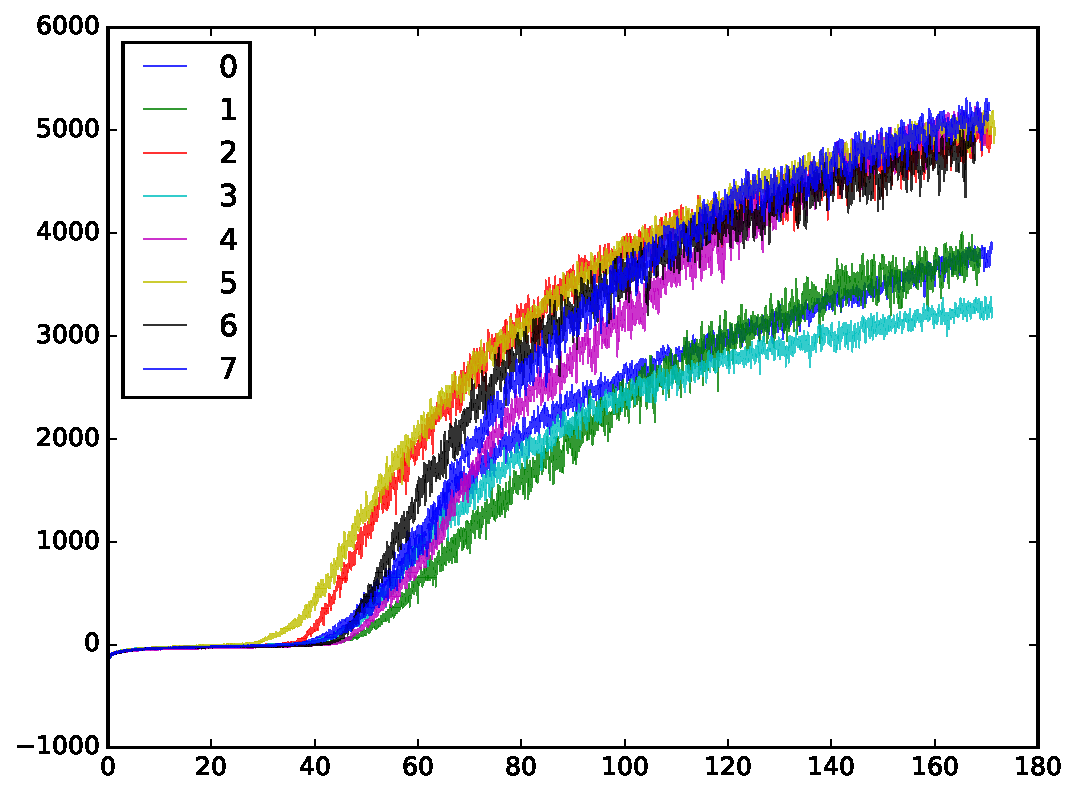
\includegraphics[width=\textwidth]{images/rec_8task_training.pdf}
	\centering
	\caption{Performance of actuator agents with domain randomization by cross-sampling initial states, the x-axis is the number of million time-steps and the y-axis is the total episode reward averaged over the last 32 episodes}\label{rec_8task_training}
\end{figure}

\subsection{Training of decider agents}
\subsubsection{Training of decision policy}
\subsubsection{Training of switcher policy}